% !TEX program = xelatex
% ============================================================
%  TROMLEORKESTRET — Technical Rider
%  Compile with:  xelatex rider.tex   (run twice)
%
%  Same design system as main.tex (the booking sheet). Sections
%  marked %%% EDIT ME are placeholders / best-guess values —
%  check and adjust before sending this out.
%
%  Overleaf: the "% !TEX program = xelatex" line above should make
%  Overleaf pick XeLaTeX automatically. If it still tries pdfLaTeX,
%  set it manually: Menu (top left) -> Settings -> Compiler -> XeLaTeX.
% ============================================================
\documentclass[10pt]{article}

% ---------- Page geometry ----------
\usepackage{geometry}
\geometry{a4paper, margin=14mm, top=12mm, bottom=9mm}

% ---------- Fonts (xelatex, system fonts) ----------
\usepackage{fontspec}
\setmainfont{Lora}[Mapping=tex-text]
\IfFontExistsTF{Bitstream Charter}
  {\newfontfamily\serifreader{Bitstream Charter}[Mapping=tex-text]}
  {\IfFontExistsTF{Charter}
    {\newfontfamily\serifreader{Charter}[Mapping=tex-text]} % macOS name
    {\newfontfamily\serifreader{XCharter}[Mapping=tex-text]}} % Linux/TeX Live name
\newfontfamily\labelfont{DejaVu Sans Condensed}[Mapping=tex-text]

% ---------- Colour palette (identical to main.tex) ----------
\usepackage[table]{xcolor}
\definecolor{bg}{HTML}{14110D}       % page background
\definecolor{cream}{HTML}{EBE2D0}    % body text
\definecolor{brightcream}{HTML}{F3E9D2} % headings / titles
\definecolor{brass}{HTML}{C59D5F}    % accent gold
\definecolor{ember}{HTML}{C1440E}    % accent rust/orange
\definecolor{muted}{HTML}{9C8A66}    % dim labels
\definecolor{bodytext}{HTML}{D8CBAF} % paragraph grey-cream
\definecolor{hairline}{HTML}{6E5F45} % faint rules

% ---------- Full-bleed dark background ----------
\newcommand{\bgfill}{%
  \begin{tikzpicture}[remember picture, overlay]
    \fill[bg] (current page.south west) rectangle (current page.north east);
  \end{tikzpicture}%
}

% ---------- Images / drawing ----------
\usepackage{graphicx}
\usepackage{tikz}
\usetikzlibrary{calc}

% ---------- Tables / lists ----------
\usepackage{array}
\usepackage{tabularx}
\usepackage{enumitem}
\usepackage{tcolorbox}
\tcbuselibrary{skins}

% ---------- Links ----------
\usepackage{hyperref}
\hypersetup{%
  colorlinks=true, urlcolor=brass, linkcolor=brass,
  pdfborder={0 0 0}, pdfborderstyle={/S/U /W 0}, hidelinks=false,
  breaklinks=true,
  pdftitle={Tromleorkestret -- Technical Rider}%
}
\hypersetup{linkbordercolor=bg, citebordercolor=bg, filebordercolor=bg, urlbordercolor=bg}
\newcommand{\cvlink}[2]{\href{#1}{\color{brass}#2}}

\setlength{\parindent}{0pt}
\setlength{\parskip}{0pt}
\pagestyle{empty}

% ---------- Small helpers (identical to main.tex) ----------
\newcommand{\eyebrow}[1]{{\labelfont\fontsize{10}{12}\selectfont\color{ember}\MakeUppercase{#1}}}
\newcommand{\rlabel}[1]{{\labelfont\fontsize{7.6}{9}\selectfont\color{brass}\MakeUppercase{#1}}}
\newcommand{\riderrow}[2]{%
  \noindent
  \begin{minipage}[t]{26mm}\rlabel{#1}\end{minipage}%
  \begin{minipage}[t]{\dimexpr\linewidth-26mm\relax}
    {\serifreader\fontsize{9.2}{13.5}\selectfont\color{bodytext}#2\par}
  \end{minipage}\\[2.6mm]%
}

\begin{document}
\color{cream}

% ================================================================
%  PAGE 1
% ================================================================
\bgfill

\noindent
\begin{tabularx}{\linewidth}{@{}X r@{}}
{\fontsize{22}{22}\selectfont\itshape\bfseries\color{brightcream} Technical Rider} &
{\labelfont\fontsize{7.6}{10}\selectfont\color{muted}\MakeUppercase{Tromleorkestret}}
\end{tabularx}\\[1mm]
{\labelfont\fontsize{9}{12}\selectfont\color{brass}\MakeUppercase{The Fire-Breathing Music Machine}}

\vspace{2mm}
{\color{brass}\hrule height 0.6pt}
\vspace{5mm}

%%% EDIT ME — one-paragraph act summary
{\serifreader\fontsize{10}{15}\selectfont\color{cream}
Tromleorkestret is a two-person live act built around a homebuilt, robotic
music machine: mechanical instruments, amplified springs and synchronised
flamethrowers, played and improvised over live. This rider covers the
stage, power, sound and safety requirements for a standard show; talk to
us ahead of time about anything unusual at your venue.\par}

\vspace{5mm}

\noindent
\begin{minipage}[t]{0.485\linewidth}

  % ---- stage & power ----                 %%% EDIT ME
  \eyebrow{Stage \& Power}\\[1mm]
  {\color{hairline}\hrule height 0.4pt}
  \vspace{1.5mm}
  \riderrow{Footprint}{L130 $\times$ W120cm (W100cm with keyboard unmounted, remounted inside the venue) $\times$ H190cm. Weight $\approx$200kg.}
  \riderrow{Surface}{Flat, solid ground --- paving, decking or a hard floor. Not suitable for grass, gravel or sand without a track/plates.}
  \riderrow{Access}{Drivable path or crane to position. Rolls up/down gentle slopes; cannot be carried up or down stairs.}
  \riderrow{Power}{Fully self-contained on internal batteries --- no venue power needed for a standard show. Multi-day festivals: trailer parking + 220V to recharge overnight.}
  \riderrow{Clearance}{$\geq$1m clear space on all sides of the machine for performers and heat/flame clearance (see Fire Safety).}

  \vspace{4mm}

  % ---- sound ----                         %%% EDIT ME
  \eyebrow{Sound}\\[1mm]
  {\color{hairline}\hrule height 0.4pt}
  \vspace{1.5mm}
  \riderrow{PA}{Own onboard PA covers small-to-mid spaces unamplified. Stereo DI line-out available if the venue system/FOH is preferred for larger spaces.}
  \riderrow{Monitoring}{Self-monitoring via onboard speakers; no separate monitor wedges required.}
  \riderrow{Mics}{None required from the venue --- all sound is generated and reinforced by the machine itself.}
  \riderrow{Soundcheck}{Not Needed - but if requested, a brief check can be done once the machine is positioned and powered.}

\end{minipage}%
\hfill
\begin{minipage}[t]{0.485\linewidth}

  % ---- fire safety ----                   %%% EDIT ME — confirm with venue's fire marshal
  \eyebrow{Pyrotechnics \& Fire Safety}\\[1mm]
  {\color{hairline}\hrule height 0.4pt}
  \vspace{1.5mm}
  \riderrow{Optional}{Fire is an optional part of the show --- we can perform a full set without it if your venue can't accommodate open flame.}
  \riderrow{Effect}{Short, controlled flame bursts (flamethrower elements) synchronised to the music --- not a pyrotechnic charge/explosive effect.}
  \riderrow{Clearance}{$\geq$4m overhead clearance from flame outlets to any flammable material. }
  \riderrow{Indoor use}{Possible with adequate ceiling height and ventilation --- must be agreed in advance and may require the venue's fire marshal / local permit sign-off.}
  \riderrow{Extinguisher}{Venue to provide one CO$_2$ fire extinguisher within reach of the performance area.}

  \vspace{4mm}

  % ---- lighting ----                      %%% EDIT ME
  \eyebrow{Lighting}\\[1mm]
  {\color{hairline}\hrule height 0.4pt}
  \vspace{1.5mm}
  \riderrow{Onboard}{The machine carries its own integrated lighting (flame glow, LEDs). No venue lighting rig is required for the show to work.}
  \riderrow{Optional}{A simple wash/key light on the performers is welcome if the venue has one, but is not essential. }

\end{minipage}

\vspace{6mm}

% ---- photo strip ----
\noindent
\begin{tikzpicture}
  \node[anchor=north west, inner sep=0pt] (p1) at (0,0)
    {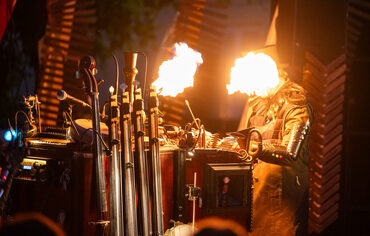
\includegraphics[width=88mm,height=40mm]{img/riderwide_crop.jpg}};
  \draw[brass, opacity=0.5, line width=0.3pt] (p1.north west) rectangle (p1.south east);

  \node[anchor=north west, inner sep=0pt, xshift=2mm] (p2) at (p1.north east)
    {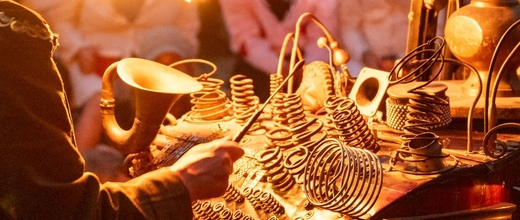
\includegraphics[width=88mm,height=40mm]{img/strip2_crop.jpg}};
  \draw[brass, opacity=0.5, line width=0.3pt] (p2.north west) rectangle (p2.south east);
\end{tikzpicture}

\vfill
{\color{hairline}\hrule height 0.4pt}
\vspace{1.5mm}
\noindent
\begin{tabularx}{\linewidth}{@{}X r@{}}
  {\labelfont\fontsize{7.2}{9}\selectfont\color{hairline} Technical enquiries: tromleorkestret@gmail.com} &
  {\labelfont\fontsize{7.2}{9}\selectfont\color{hairline} 01 / 02}
\end{tabularx}

\clearpage

% ================================================================
%  PAGE 2
% ================================================================
\bgfill

\noindent
\begin{tabularx}{\linewidth}{@{}X r@{}}
{\fontsize{19}{19}\selectfont\itshape\bfseries\color{brightcream} Schedule, Crew \& Hospitality} &
{\labelfont\fontsize{7.6}{10}\selectfont\color{muted}\MakeUppercase{Tromleorkestret --- Technical Rider}}
\end{tabularx}

\vspace{2mm}
{\color{brass}\hrule height 0.6pt}
\vspace{6mm}

\noindent
\begin{minipage}[t]{0.485\linewidth}

  % ---- load-in / schedule ----            %%% EDIT ME — confirm timings
  \eyebrow{Load-In \& Schedule}\\[1mm]
  {\color{hairline}\hrule height 0.4pt}
  \vspace{1.5mm}
  \riderrow{Load-in}{$\approx$45--60 minutes from vehicle to stage-ready, given clear drivable access.}
  \riderrow{Soundcheck}{15--20 minutes.}
  \riderrow{Show length}{Flexible --- typically 30--60 minutes; can be adapted to your slot.}
  \riderrow{Load-out}{$\approx$30--45 minutes.}
  \riderrow{Turnaround}{For multiple sets/days, the machine needs $\approx$1 hour between shows to refuel and reset.}

  \vspace{4mm}

  % ---- crew ----                          %%% EDIT ME
  \eyebrow{Crew}\\[1mm]
  {\color{hairline}\hrule height 0.4pt}
  \vspace{1.5mm}
  \riderrow{Touring party}{2 (performers, self-sufficient on technical setup).}
  \riderrow{Local crew}{None required for load-in/out under normal access conditions; 1 extra pair of hands appreciated if access is difficult (stairs, long carry, etc.).}
  \riderrow{Parking}{Parking for car + trailer for the duration of the show --- preferably without needing to disconnect them --- with clear space behind the trailer to unload.}

\end{minipage}%
\hfill
\begin{minipage}[t]{0.42\linewidth}

  % ---- hospitality ----                   %%% EDIT ME
  \eyebrow{Hospitality}\\[1mm]
  {\color{hairline}\hrule height 0.4pt}
  \vspace{1.5mm}
  \riderrow{Catering}{Full catering incl. vegetarian option, and beverages with and without alcohol.}
  \riderrow{Dressing room}{A private, lockable space to change and store cases, close to the stage.}
  \riderrow{Lodging}{Free accommodation for overnight/multi-day bookings.}

\end{minipage}

\vspace{6mm}

% ---- photo strip ----
\noindent
\begin{tikzpicture}
  \node[anchor=north west, inner sep=0pt] (r1) at (0,0)
    {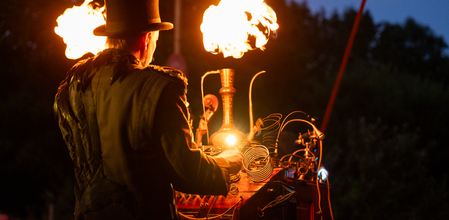
\includegraphics[width=57mm,height=28mm]{img/strip4_crop.jpg}};
  \draw[brass, opacity=0.5, line width=0.3pt] (r1.north west) rectangle (r1.south east);

  \node[anchor=north west, inner sep=0pt, xshift=2mm] (r2) at (r1.north east)
    {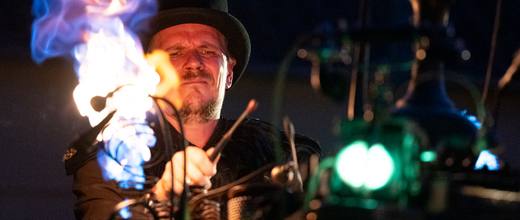
\includegraphics[width=66mm,height=28mm]{img/strip5_crop.jpg}};
  \draw[brass, opacity=0.5, line width=0.3pt] (r2.north west) rectangle (r2.south east);

  \node[anchor=north west, inner sep=0pt, xshift=2mm] (r3) at (r2.north east)
    {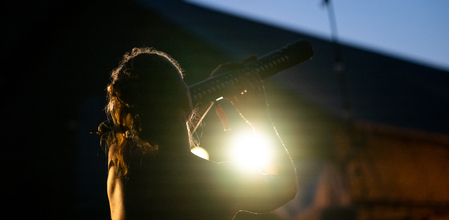
\includegraphics[width=57mm,height=28mm]{img/strip6_crop.jpg}};
  \draw[brass, opacity=0.5, line width=0.3pt] (r3.north west) rectangle (r3.south east);
\end{tikzpicture}

\vspace{5mm}

% ---- contact block ----              (identical to main.tex)
\noindent
\begin{tcolorbox}[
    enhanced, colback=brass!8!bg, colframe=brass!55, boxrule=0.5pt,
    arc=0pt, left=5mm, right=5mm, top=3.5mm, bottom=3.5mm
  ]
  \begin{tabularx}{\linewidth}{@{}X r@{}}
    \begin{minipage}[c]{0.6\linewidth}
      {\fontsize{12.5}{14}\selectfont\itshape\bfseries\color{brightcream} Tromleorkestret}\\[0.8mm]
      {\labelfont\fontsize{7.6}{11}\selectfont\color{muted}
       Att. Hjalte Bested Hjorth \textperiodcentered\ Bj\o rnekloen 374 st.tv,
       1440 K\o benhavn K \textperiodcentered\ CVR 37165107}
    \end{minipage}
    &
    \begin{minipage}[c]{0.38\linewidth}
      \raggedleft
      {\labelfont\fontsize{8}{15}\selectfont\color{cream}
       \cvlink{mailto:tromleorkestret@gmail.com}{tromleorkestret@gmail.com}\\
       \cvlink{tel:+4523282926}{+45 23 28 29 26}\\
       \cvlink{https://tromleorkestret.com}{tromleorkestret.com}\\
       \cvlink{https://instagram.com/tromleorkestret}{Instagram} \textperiodcentered\
       \cvlink{https://facebook.com/tromleorkestret}{Facebook} \textperiodcentered\
       \cvlink{https://youtube.com/@tromleorkestret}{YouTube}}
    \end{minipage}
  \end{tabularx}
\end{tcolorbox}

\vfill
{\color{hairline}\hrule height 0.4pt}
\vspace{1.5mm}
\noindent
\begin{tabularx}{\linewidth}{@{}X r@{}}
  {\labelfont\fontsize{7.2}{9}\selectfont\color{hairline} Technical enquiries: tromleorkestret@gmail.com} &
  {\labelfont\fontsize{7.2}{9}\selectfont\color{hairline} 02 / 02}
\end{tabularx}

\end{document}
